%! Author = yadielperez
%! Date = 4/3/21

\documentclass{article}[draft]
\usepackage{blindtext}
\usepackage{graphicx}

\title{Phase 2}
\date{2021\\February}

\author{Gabriel L., Jose Lazcano, Jesus Jaime,\\ Yadiel Perez, Fernando, Cristian}

\begin{document}

\maketitle
\section{Name, Place and Date}
ZeitNehmer Workflow Manager\\
Mayaguez, PR\\
April 5, 2021
\section{Current Situation, Needs, Ideas and Concept}
\vspace{10pt}
The front-end of our project has started to take shape. For the most part the front-end is mostly finished just needing a couple final changes that can be handled in a future sprint. Users can now register and login to the website. This is all maintained in an database and is kept even when the Django server is restarted. Work on the back-end has begun as we start to whittle away at the interface we want for the users and as we begin to plan out how we're going to handle managers and users access to parts of the website.
\\

Managers need project management programs to manage their employees tasks and projects and give them a way for them to know what they need to do. Most of these programs have become bloated over time and have overcomplicated tasks that should be pretty straightforward causing the need for managers to take training to be able to use these tools. The project would involved in creating a project management program that cuts the bloat and focuses on making an intuitive and easy to use platform where no training is needed to properly use. This would involve a structure where:
\begin{enumerate}
\item Platform for managers: Managers can access a platform to view tasks and projects and delegate them to employees.
\item Platform for employees: Employees can view tasks assigned to them and add notes alerting the manager of questions and or detailed info about the task.
\end{enumerate}
\section{Scope, Span and Synopsis}
\vspace{10pt}
The problem is to understand project management in general: deadlines, task lists, schedules, file sharing, communication, teamwork, and logistics of project management. This is used to build a theory of management systems: leadership, planning, project monitoring, status, standards and, improvement.

The project is to develop and research a Program Management Software. This project is expected to cover:
\begin{enumerate}
    \item project monitoring: team performance, task duration
    \item team collaboration
    \item task management: prioritize, strategic planning,  scheduling
    \item reporting
\end{enumerate}

\section{Assumptions and Dependencies}
\vspace{10pt}
Rough sketch requirements as user stories:
\begin{quotation}
    As a user, having an organized and productive workflow is very critical and important, because it drastically improves the productivity of the user and the company. When its time to divide the work withing a team or assigning work to your employees having a Workflow management app really helps the process. If someone is stuck in a task, they can show it on the app, so a manager/Leader can send him a message and start helping them. The employee/manager and the team-member/Leader communication improves by having the online message system.
\end{quotation}
\begin{quotation}
    As a user, having an easy-to-use and accessible Workflow Management app can be really helpful. I would like to be able to create and edit workflows as easy as possible, and to be remained about deadlines, messages and updates.
\end{quotation}

\section{Implicit/Derivative Goals}
\vspace{10pt}

Domain Requirements:
\begin{itemize}
    \item The data base must store end-user accounts, along with their password and personal information needed to create an account.
    \item The end-user should be able to create, edit, and delete current or new workflows.
    \item The end-user should be able to edit, update or delete their personal information from the data-base.
    \item The app should hide the personal information given by creating an account unless the end-user require it.
    \item The system-to-be needs to keep a list of every user registered so it can quickly identify if the user haves an account or it needs to create one.
    \item System-to-be must identify the user ``rank'' in order to classify the account as the manager or employee, as a leader or as a teammate.
    \item System-to-be must detect if end-user is active in on the page, for an online symbol that identify to other people that you are currently on the app and they can message you.
    \item System-to-be must detect \& update the status of the task every time a user makes an update on their workflow.
    \item System-to-be must send push notification to the users notifying the deadlines, updates and messages.
\end{itemize}
\vspace{30pt}
Interface Requirements:

\begin{itemize}
    \item The system-to-be has a downtime of 15 minutes every 24 hours for a backup to save any changes of the website from the users, and storing important information on the data base.
    \item The system-to-be must store every workflow created in the data-base and update the ones that where changed.
    \item The system-to-be must show the workflows that are already stored, so end-users can identify and select witch one they want to work on.
    \item For security of the end-user account, the password should be initially obscured. They should have an option that enables the password to show for reviewing purposes.
\end{itemize}
For the system to work properly and ensure a good experience with the users it must comply with the following:
\begin{enumerate}
  \item Changes made will be updated at real time or with no more than a 200 ms delay for 99\% of the cases.
  \item Users will be notified about changes relating to their tasks as soon as it is updated.
  \item Even at peak times server load should be lower than 80\%
  \item Response times from interface must be kept lower than 500 ms.
  \item Platform must be available at all times, with the exclusion of programmed downtimes.
\end{enumerate}

\vspace{70pt}
Software Structure:

\begin{itemize}
    \item Security:

\vspace{5pt}
The Software will have the implementation of account registration, Users will provide an email and set up their accounts,
setting their password as Username. Once the account has been created and the User has logged in, User must select the
kind of work they will be focusing on and manage from available options. This includes:
\begin{enumerate}
    \item Sales
    \item Creative
    \item Marketing
    \item IT
    \item Finance
    \item Customer Service
    \item Software Development
    \item ECT
    \item Manufacturing
\end{enumerate}
Once
User has chosen their work, a link will be generated to invite other users to join on the workflow, input information
regarding the workflow.\\
\end{itemize}

\begin{itemize}
    \item Data Management:

    \vspace{5pt}
    Users also can Customize their main UI Workstation and save their settings
    Users can add widgets and tools to their
    work station
    The System tracks current events and their current status, from Ongoing to Complete.
    The System tracks Current Users that are online and their current workflows.
    System Monitors and sends notifications accordingly to constantly update the status of workflow.
\end{itemize}

\begin{itemize}
    \item Report Generation

    \vspace{5pt}
    TheSystem will track and report on the different workflows.
    This data is sent to the different users to their corresponding workflows.
    Users can
    update their workflows and report on their current state of their events.
    Messages can be sent to other users.
\end{itemize}
\vspace{5pt}
Domain Entities:
\begin{quotation}
    The entities methods take care of the invariants and rules of the entity instead of having those rules spread across the application layer.
    Every class has in own attributes and methods that will be called when the application is running but keeps it in an organized matter.
\end{quotation}
\bigbreak
\begin{figure}[ht!]
    \centering
   % \includegraphics[width=1.2\columnwidth]{Images/Domain_Entities.pdf}
    \caption{Domain Entities}
    \label{fig:figure}
\end{figure}
\bigbreak
Domain Functions:
\begin{quotation}
    The domain functions takes care of the data when classes or variables get called when the user interacts with the platform.
    We can see this in the diagram below where we can view the navigation of the data between entities.
\end{quotation}
\bigbreak
\begin{figure}[ht!]
    \centering
%    \includegraphics[width=0.5\columnwidth]{Images/state-view.pdf}
    \caption{Domain Entities}
    \label{fig:figure2}
\end{figure}
\bigbreak
\noindent Software Component Design:
\bigbreak
\noindent \textbf{module workflows:}
\begin{quote}
  \textbf{Variables:}
  \begin{quote}
    workflowName \textbf{String}; workflowDescription \textbf{String}; members \textbf{List}
  \end{quote}
  \textbf{Functions:}
  \begin{quote}

    status: boolean, status()
    \begin{quote}
      updates workflow current status, returns "ongoing" or "completed"
    \end{quote}

    currentlyOnline: List, currentlyOnline()
    \begin{quote}
      returns all users who are assigned to this task and are online.
    \end{quote}

    updateDescription: null, updateDescription(workflowDescriptions)
    \begin{quote}
     changes the workflow description.
    \end{quote}
  \end{quote}
\end{quote}
\textbf{end module}
\bigbreak

\noindent \textbf{module workflowManagement:}
\begin{quote}
  \textbf{Variables:}
  \begin{quote}
    username \textbf{String}; isManager \textbf{boolean}
  \end{quote}

  \textbf{Functions:}
  \begin{quote}

    createWorkflow: null, createWorkflow(isManager)
    \begin{quote}
      a new workflow is created, user must be a manager to do so.
    \end{quote}

    viewWorkflow: List, viewWorkflow(username, isManager)
    \begin{quote}
      views all workflows a certain user is currently on, must be a manager.
    \end{quote}

    onlineMembers: List, onlineMembers()
    \begin{quote}
      returns all members who are currently active.
    \end{quote}

  \end{quote}
\end{quote}
\textbf{end module}
\bigbreak

\noindent \textbf{module notifications:}
\begin{quote}
  \textbf{Variables:}
  \begin{quote}
    workflowName \textbf{String}; workflowMembers \textbf{List}
  \end{quote}

  \textbf{Functions:}
  \begin{quote}

    workflowUpdated: null, workFlowUpdated(workflowMembers, workflowName)
    \begin{quote}
      notifies all workflow memebers a change hasbeen made or status has changed.
    \end{quote}

    newWorkflow: null newWorkflow(workflowMembers)
    \begin{quote}
      notifies all members of the workflow that it has been created.
    \end{quote}

  \end{quote}
\end{quote}
\textbf{end module}
\bigbreak

\noindent \textbf{module accounts:}
\begin{quote}

  \textbf{Variables:}
  \begin{quote}
    email \textbf{String}; username \textbf{String}; department \textbf{String}; isManager \textbf{boolean}
  \end{quote}
  \textbf{Functions:}
  \begin{quote}

    changeDepartment: null, changeDepartment(department)
    \begin{quote}
      Switchs the user current department.
    \end{quote}


    managerStatus: boolean, managerStatus(isManager)
    \begin{quote}
      Assigns the user as a manager or as a regular user, returns manager status.
    \end{quote}

  \end{quote}
\end{quote}
\textbf{end module}
\section{Features}
After various consideration and to streamline the creation of the main feature (workflows) it is important to complete a feature first, which is users accounts. Users accounts can be defined as the user's passport for accesing the features the program offers, these are created by each user and each of them must be unique. This is important because it will be key on features such as:
\begin{enumerate}
  \item Workflow access and assignment.
  \item Roles on workflows
  \item Teams
\end{enumerate}
These are just a rough example of features that require accounts to work at their fullest, more details will be given once they will be worked on.
\vspace{10}

In order for users to access our services they must own an account or create one. With this requirement in mind, the process can be resumed by the following diagram:

\begin{figure}[h!]
    \centering
    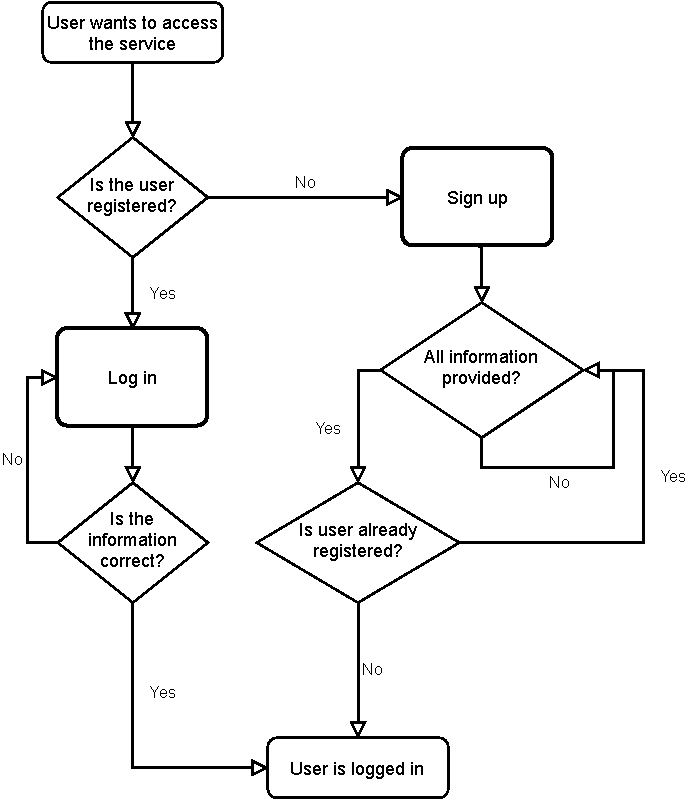
\includegraphics[scale=0.75]{Images/AccessDiagram.pdf}
    \caption{Accesss Diagram}
    \label{fig: figure 1}
\end{figure}

\vspace{200}

To maintain simplicity this process can be divided into different components, these are:

\begin{enumerate}
  \item Sign up
  \item Log in
  \item Users
  \item Registration
\end{enumerate}


\section{Sign-Up}
  In order for the user to create an account for now an username and password must be provided, also the password must be confirmed. For the account to be succesfully created the username te user provides must not be the same as any in the database, and the password and password confirmation must match. A sketch as been made that includes:
  \begin{itemize}
    \item A textbox to add the username
    \item A textbox to add a password
    \item A list of some current limitations of the password requirements.
    \item A textbox to confirm the previous password.
  \end{itemize}

  \begin{figure}[h!]
      \centering
      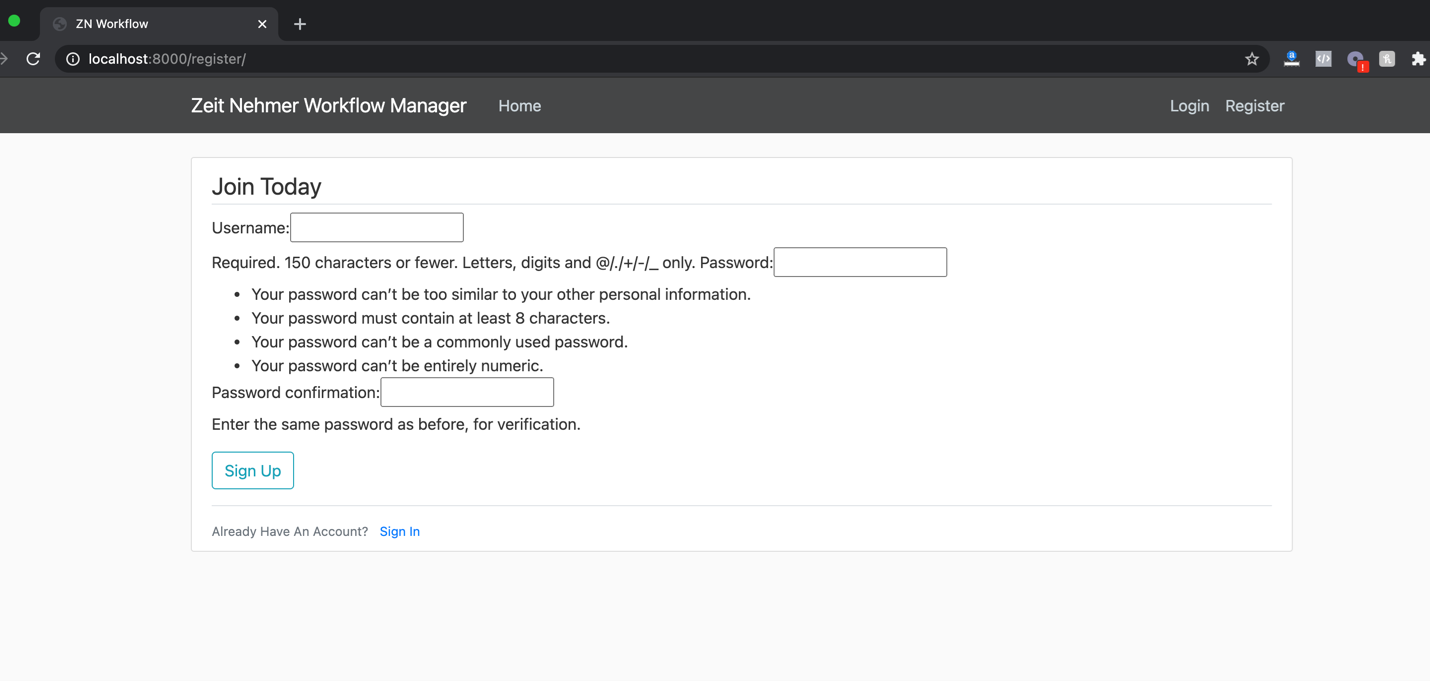
\includegraphics[scale=0.75]{Images/signupMock}
      \caption{Sign Up interface}
      \label{fig:figure 2}
  \end{figure}

\section{Log-In}

  In order for users to access their workflows they will need to log in into their created accounts. This will help keep their workflows secured, since only them and their assigned members will be able to access them.

  \subsection{Implementation}

  Existing users can use their credentials to log into the app, this will be an email or username and a password. The login mechanism uses the users registered with the sign up form to enter the app as an existing user, this is confirmed using the database so that both the email/username and password combination match with the ones registered on the database, if it fails the user will be asked to enter their information again. Once sucessful the user will be able to access all of their content.

  \subsection{User Interface}
\begin{figure}[h!]
     \centering
      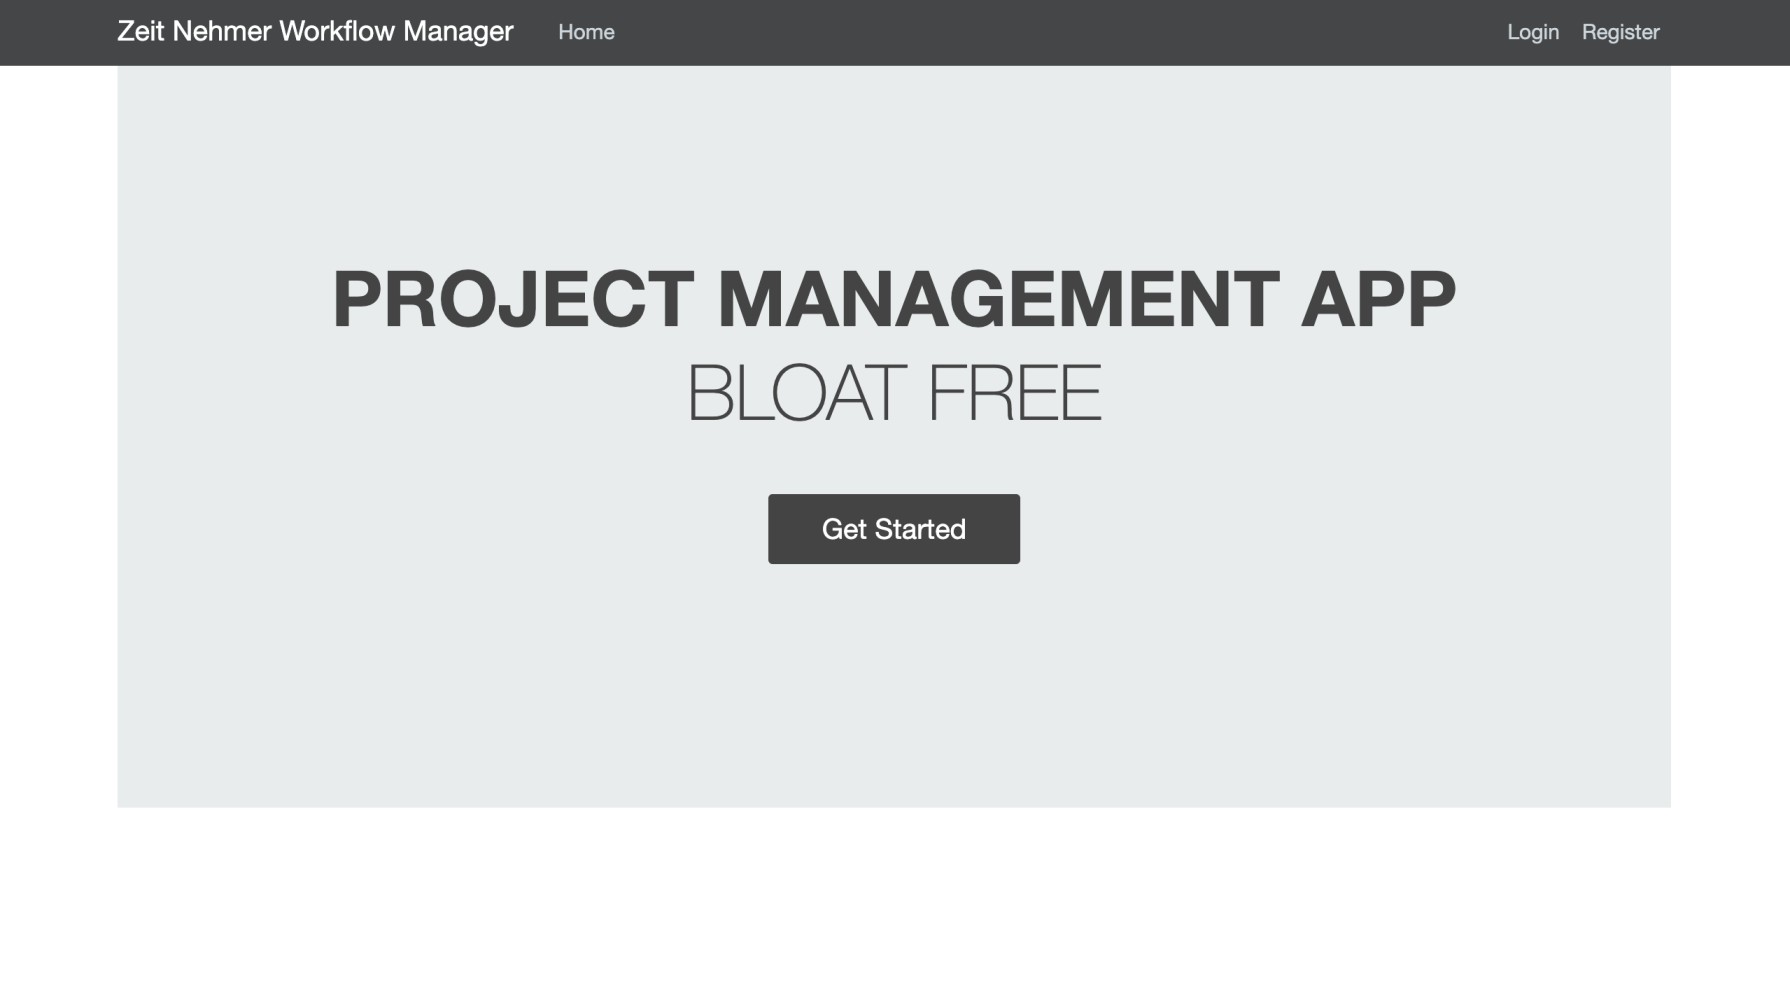
\includegraphics[width=1.2\columnwidth]{Images/homepage.jpg}
      \caption{Home Page}
      \label{fig:figure 3}
\end{figure}

  \begin{enumerate}
    \item A textbox to add the email or username
    \item A textbox to add the user's password
    \item A button to continue with the login
    \item A "Sign up" button in case the user is a new member, this will redirect the user to the sign up procedure discussed before.
  \end{enumerate}
In Figure 6 a prototype of what will be our login page is presented, this includes:
  \begin{figure}[h!]
      \centering
      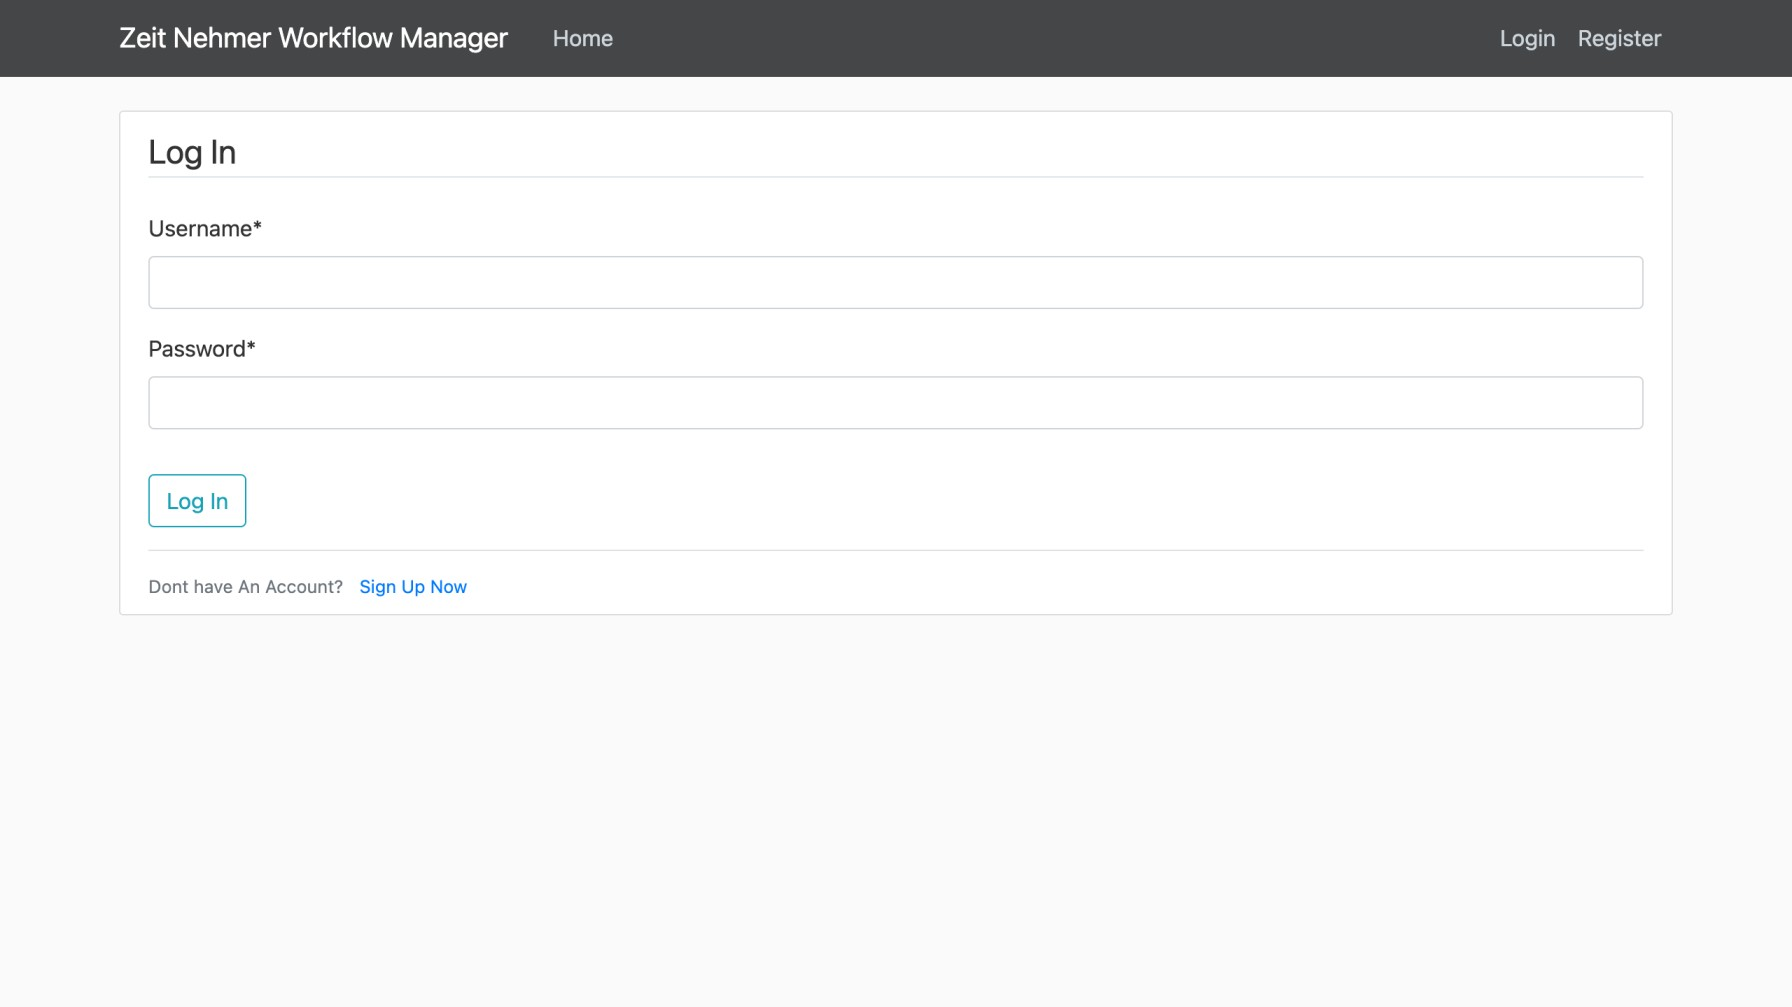
\includegraphics[width=1.2\columnwidth]{Images/LogIn.jpg}
      \caption{Log In interface}
      \label{fig:figure 4}
  \end{figure}

  In order for the user to not lose their account and to minimize that they make another one, a "Forgot password?" button will be added. There an email will be sent to the provided email and a procedure to reset the password will take place. This will be worked on a future sprint.


\section{Users}
  Users can be defined as the people who have made an account and use our platform. There are still some doubts on how this is going to be handle, one of the option is the use of Object Oriented Programming (OOP). These users can be divided intro categories:
  \begin{enumerate}
    \item Administrators
    \begin{quote}
        These users can administrate other users as well as give and take permissions. They will be able to login in a separate from as normal users, like on Figure 5.
        \begin{figure}[h!]
            \centering
            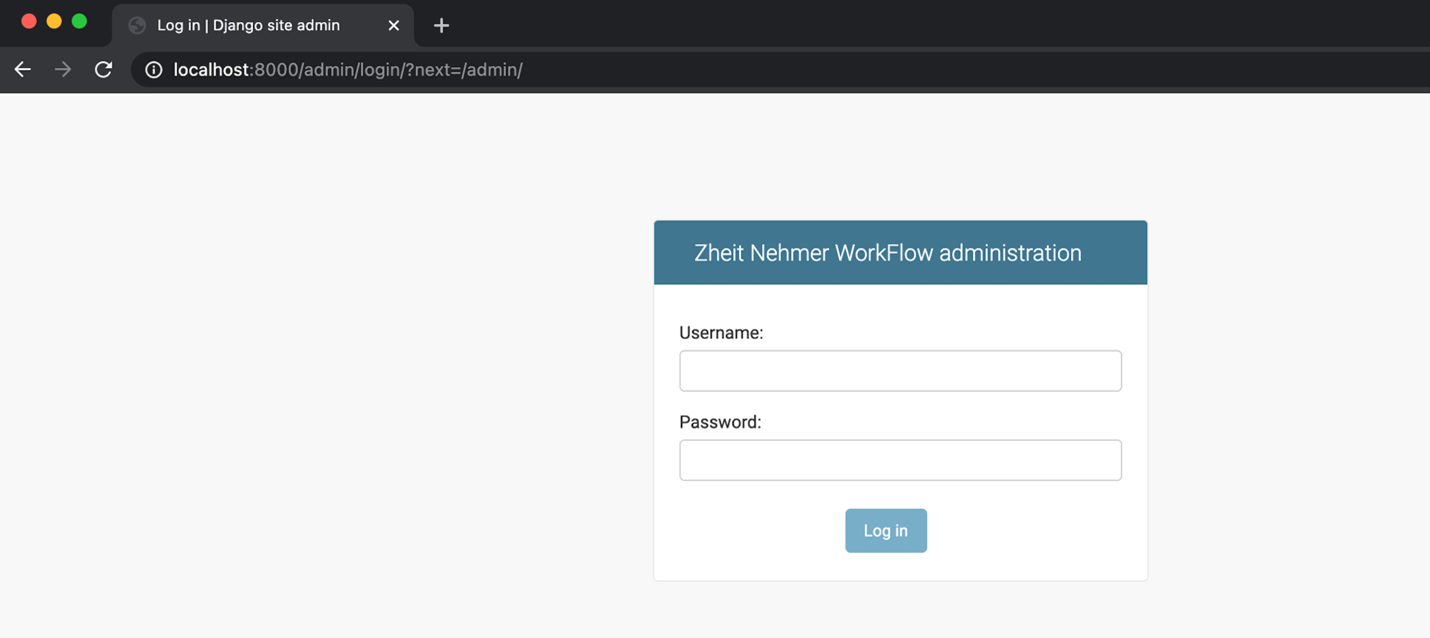
\includegraphics[scale=0.75]{Images/adminLogin.png}
            \caption{Admin Registration}
            \label{fig:figure 5}
        \end{figure}

        \vspace{160}

        This will take the administrator to a management area.

        \begin{figure}[h!]
            \centering
            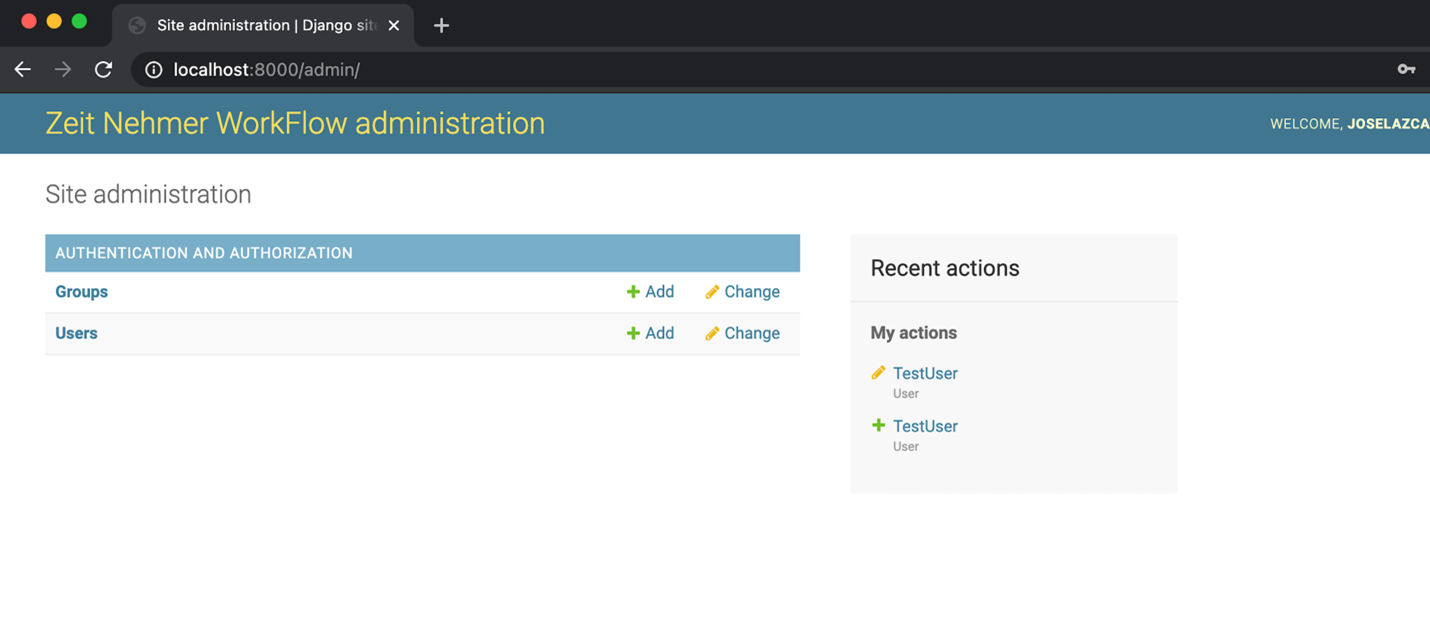
\includegraphics[scale=0.75]{Images/adminManage.png}
            \caption{Administrator Management}
            \label{fig:figure 6}
        \end{figure}



        An administrator can give permissions to users such as:
        \begin{itemize}
          \item Active: decides whether or not the account should have access to the website.
          \item Staff Status: designates whether the user can log into the admin site.
          \item Superuser status: designates that this user has all permissions without assigning them.
        \end{itemize}

        An example of how this permissions will be managed is presented next.

        \begin{figure}[h!]
            \centering
            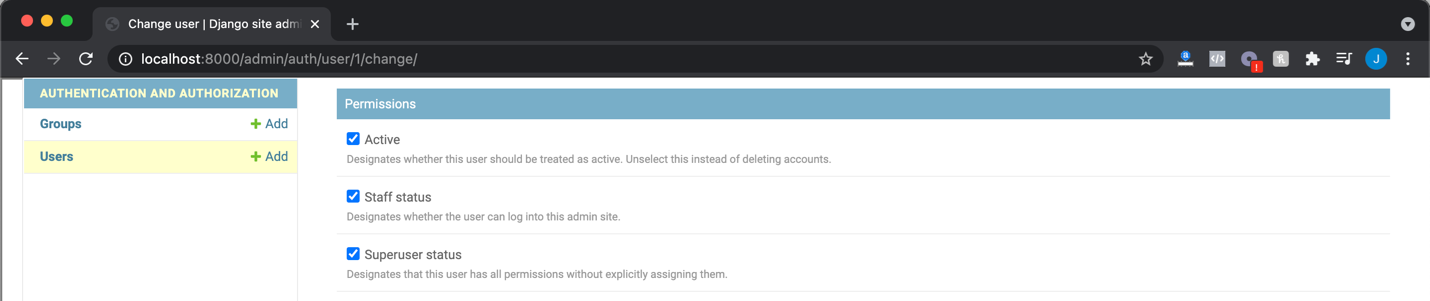
\includegraphics[width=1.2\columnwidth]{Images/adminPerm.png}
            \caption{Administrator Permissions}
            \label{fig:figure 7}
        \end{figure}

        \vspace{100}

        And administrator can also individualy assign or take permissions, such as the next example.

        \begin{figure}[h!]
            \centering
            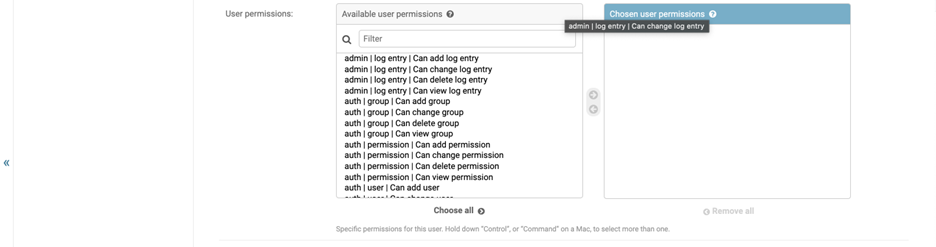
\includegraphics[width=1.2\columnwidth]{Images/adminPerm2.png}
            \caption{Administrator Individual Permissions}
            \label{fig:figure 8}
        \end{figure}
    \end{quote}

    \item Superuser
    \begin{quote}
      A user with all permissions available given.
    \end{quote}

    \item User
    \begin{quote}
      A regular user with the essentials permissions given.
    \end{quote}
  \end{enumerate}

\section{Registration}
The user inputs his data and log in credentials, the system must detect that this is a new account and that information such as email are not already in used by an existing account. If this the case the user will not be able to sign up and will be require to update the information in order to continue. Once succesfull, the system will save the username, password and email into the corresponging user category (Eg. admin, manager or user). There are some elements to take in consideration at the time of registration such as:
\begin{enumerate}
  \item Demographics

  \item Username
  \begin{quote}
    It is important that to no ther user has the same username since this can cause confusion and the server would save two password under the same username.
  \end{quote}

  \item Validation
  \begin{quote}
    The system should verify the user has been able to register without problem and that the username and password combination can be use to access the platform at any time.
  \end{quote}

  \item Password Strength
  \begin{quote}
    The user must be asked to provide a strong password to maintain security at a high level, it must not be the same as the username or any personal information.
  \end{quote}

  \item Group Selection
  \begin{quote}
    If the user has been invited to a group once registered he should be able to accept the invitation and access the group's workflow without problem.
  \end{quote}
\end{enumerate}
\section{Workflows}
In order to create a new workflow, you fill the following fields:
\begin{enumerate}
    \item Workflow Name
    \item Description
    \item Due Date
    \item Workflow Priority(Low, Medium, Urgent)
\end{enumerate}
\begin{figure}[h!]
            \centering
            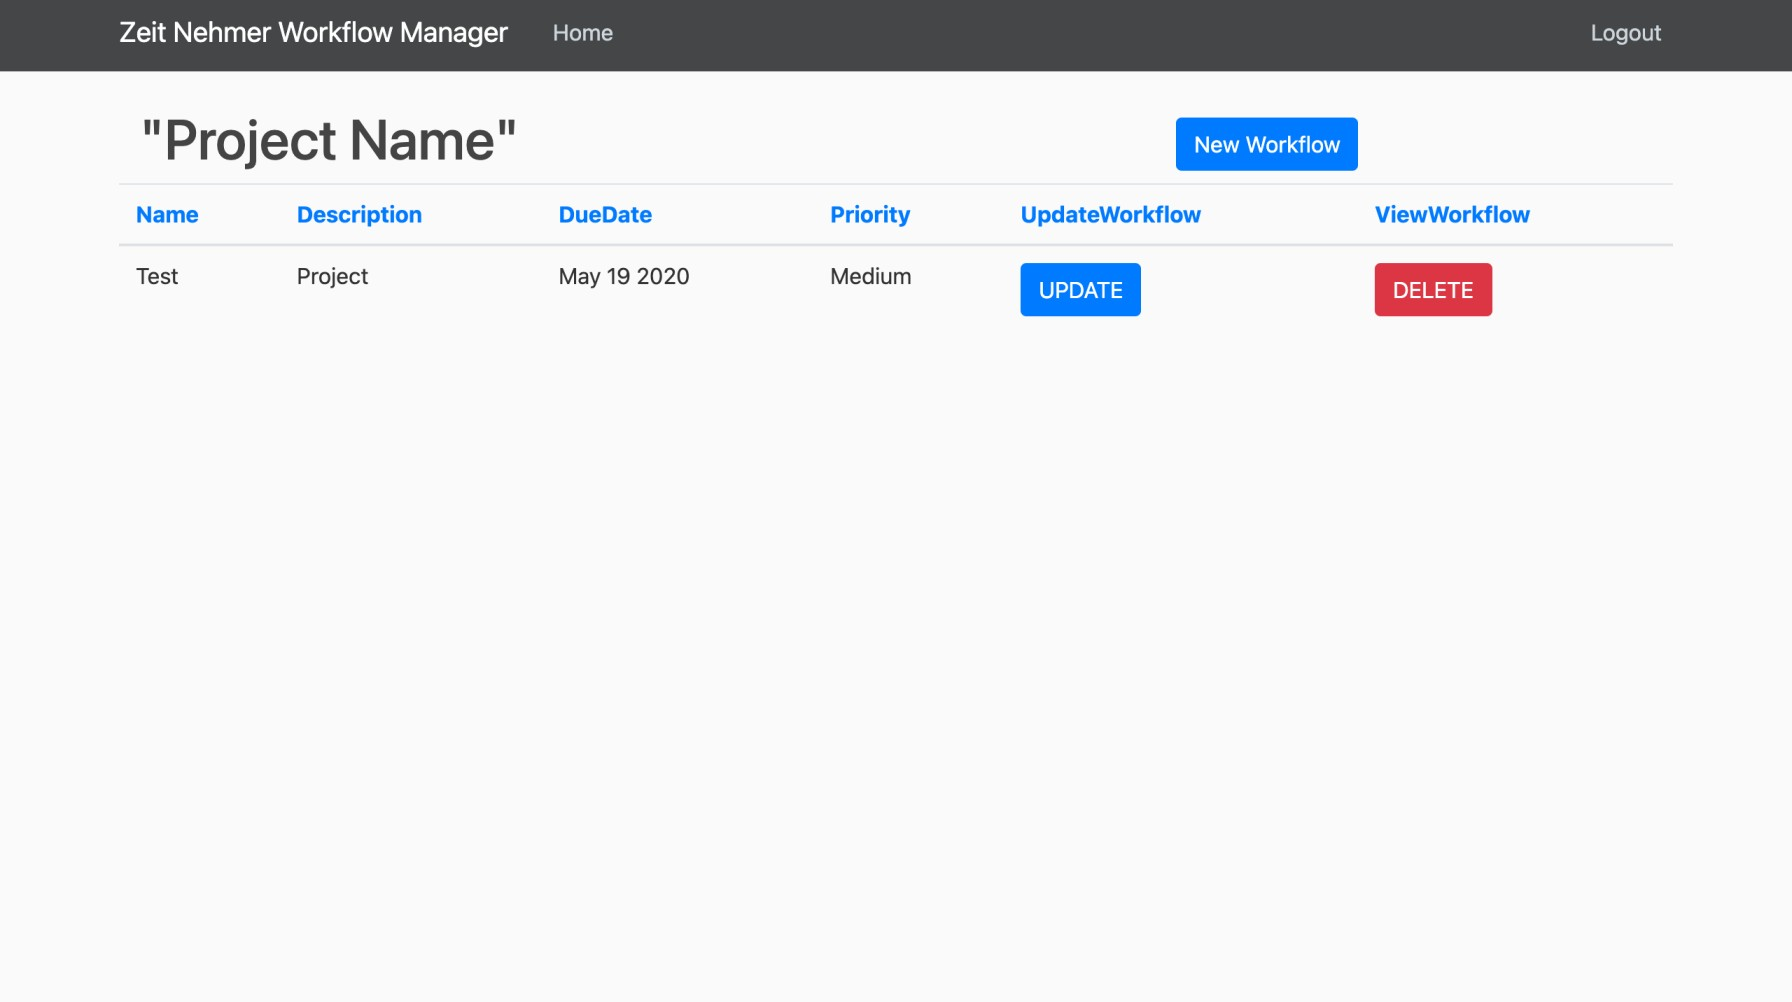
\includegraphics[width=1.2\columnwidth]{Images/Workflows.jpg}
            \caption{User Workflows}
            \label{fig:figure 9}
        \end{figure}
This workflows have the CRUD functionalities:
\begin{enumerate}
    \item Create
    \item Read
    \item Update
    \item Delete
\end{enumerate}





\section{Terminology}
\begin{center}

    \begin{tabular}{| l | p{5cm} |}\hline
    Term & Short definition \\ \hline
    Event & This can be referred as a task or job that the User has access to. \\ \hline
    User & Subject that enters and interacts with the system. \\ \hline
    System & This specifically refers to the software itself. \\ \hline
    UI & User Interface; Everything that the Users can see on display on the system. \\ \hline
    Workstation & The Workstation is the main User Interface where one will manage, access and configure the Users Workflow. \\ \hline
    Workflow & Page where all the social, working and management takes place. Each group provides workflows for each individual type ( sales
    , T I, ...). \\ \hline
    Social Integration & Provides social interaction between group members and users across the platform. Making the work environment very interactive
    and easier to use. \\ \hline
    Rank & A category assigned to the User. (i.e Manager, Student, Profesor, Employee). \\ \hline
    Downtime & A period of time when the platform is not available. \\ \hline
    \end{tabular}

\end{center}
\section{Roles}
\vspace{10pt}
\begin{center}

\begin{tabular}{| l | p{5cm} |}\hline
Name & Main Role \\ \hline
Gabriel L. & fetching information from the data-base\\ \hline
Yadiel     & Back-End\\ \hline
Cristian   & Front-end-design \\ \hline
Fernando   & Back-End \\ \hline
Jesus	   & Information storage\\ \hline
Jose Lazcano  & User Interface \\ \hline
\end{tabular}

\end{center}
\end{document}
